% !TEX encoding = UTF-8 Unicode
% !TEX root = BioInspired.tex

%%%  This is the main driver file.   It is mostly a list of file includes.   Read through and edit as needed.

\documentclass[table]{book}

\usepackage{listings}
\usepackage{color}

\definecolor{dkgreen}{rgb}{0,0.6,0}
\definecolor{gray}{rgb}{0.5,0.5,0.5}
\definecolor{mauve}{rgb}{0.58,0,0.82}

\lstset{frame=tb,
  language=Python,
  aboveskip=3mm,
  belowskip=3mm,
  showstringspaces=false,
  columns=flexible,
  basicstyle={\small\ttfamily},
  numbers=none,
  numberstyle=\tiny\color{gray},
  keywordstyle=\color{blue},
  commentstyle=\color{dkgreen},
  stringstyle=\color{mauve},
  breaklines=true,
  breakatwhitespace=true,
  tabsize=3
}

\usepackage[width=6.5in, height=9.0in, top=1.0in, papersize={8.5in,11in}]{geometry}
\usepackage[pdftex]{graphicx}
\DeclareGraphicsExtensions{.pdf,.png,.jpg}
%\usepackage{draftwatermark}
\usepackage{amsmath}
\usepackage{amsthm}
\usepackage{amssymb}
%\usepackage{txfonts}
\usepackage{textcomp}
%\usepackage{amsthm}
%\usepackage{array}
%\usepackage{datetime}
\usepackage{anyfontsize}
\usepackage{t1enc}
\usepackage[section,subsection]{extraplaceins}   %%%  \FloatBarrier
\usepackage[all]{xy}
\usepackage{fancyhdr}
\usepackage{hyperref}
\usepackage{verbatim}
\usepackage{algorithm}
\usepackage{makeidx}
\usepackage{multicol}
\usepackage{multirow}
\usepackage{color}
\usepackage{rotating}
\usepackage{wrapfig}
\usepackage{tikz}
\usetikzlibrary{shapes.geometric, arrows}
%\usepackage{tabularx}
\usepackage{xcolor}
\usepackage{framed}
\usepackage{xspace}
\usepackage{listings}
\lstset{language=python,frame=ltrb,framesep=5pt,basicstyle=\normalsize,
 keywordstyle=\ttfamily\color{DarkRed},
%morecomment=[n][\textbf]{In\ [}{]\:},
%morecomment=[n][\textbf]{Out\ [}{]\:},
morecomment=[s][\color{blue}]{In\ [}{]\:},
morecomment=[s][\color{red}]{Out[}{]\:},
identifierstyle=\ttfamily\color{DarkBlue}\bfseries,
commentstyle=\color{OliveGreen},
stringstyle=\ttfamily,
showstringspaces=false,tabsize = 3}

\lstdefinelanguage{shell} {
commentstyle = \color{black},
keywordstyle = \color{black},
stringstyle = \color{black},
identifierstyle = \color{black},
morecomment=[s][\color{blue}]{In\ [}{]\:},
morecomment=[s][\color{red}]{Out[}{]\:},
 }

\newtheorem{thrm}{Theorem}
\newtheorem{lem}[thrm]{Lemma}
\newtheorem{cor}[thrm]{Corollary}
\newtheorem{rem}[thrm]{Remark}
\newtheorem{defn}[thrm]{Definition}
\newtheorem{exmpl}[thrm]{Example}

% this gives a little box for the end of a proof:
%
\def\endthrmbox{$\sqsubset \!\!\!\! \sqsupset$}

\newcommand{\dis}{\displaystyle}
 \def      \RR             {{\mathbb R}} 
        \def      \NN             {{\Bbb N}} 
        \def      \QQ             {{\Bbb Q}} 
        \def      \CC             {{\Bbb C}} 
        \def      \ZZ             {{\Bbb Z}} 
 
 
        \def       \a              {{\alpha}} 
        \def       \b              {{\beta}} 
        \def       \d              {{\delta}} 
        \def       \D              {{\Delta}} 
        \def         \e              {{\varepsilon}} 
        \def         \g              {{\gamma}} 
        \def         \G              {{\Gamma}} 
        \def       \l              {{\lambda}} 
        \def       \L              {{\Lambda}} 
        \def        \m               {{\mu}} 
        \def         \n              {{\nabla}} 
        \def       \var          {{\varphi}} 
        \def         \s              {{\sigma}} 
        \def       \Sig          {{\Sigma}} 
        \def       \Om          {{\Omega}} 
 
        \def       \t              {{\tau}} 
        \def         \th             {{\theta}} 
        \def       \O              {{\Omega}} 
        \def       \o              {{\omega}} 
        \def         \z              {{\zeta}} 
       \def        \P             {{\Phi}} 
       \def        \p             {{\phi}} 
        %Other macros 
 
        \def       \iy              {{\infty}} 
        \def         \pa             {{\partial}} 
        \def         \div           {{\rm div}} 
         \def       \na            {{\nabla}} 
 



\newcommand{\pythonlogo}{
\\[-2mm] \begin{picture}(0,0)
\put(-40,-40){\includegraphics[scale=0.25]{./Figures/pythonlogo.png}}
\end{picture}
}

\newcommand{\clogo}{
\\[-2mm] \begin{picture}(0,0)
\put(-30,-30){\includegraphics[scale=0.2]{./Figures/clogo.png}}
\end{picture}
}

\newcommand{\roslogo}{
\\[-2mm] 
\begin{picture}(0,0)
\put(-30,-30){\includegraphics[scale=0.2]{./Figures/roslogo.png}}
\end{picture}
}


\tikzstyle{master} = [rectangle, draw, text width=6em, text centered, minimum
height=3em]
\tikzstyle{node} = [rectangle, draw, text width=6em, text centered, rounded
corners, minimum height=3em]

\newtheorem{summary}{Summary:}
\newtheorem{example}{Example:}[section]

\definecolor{OliveGreen}{cmyk}{0.64,0,0.95,0.40}
\definecolor{DarkBlue}{cmyk}{0.76,0.76,0,0.20}
\definecolor{DarkRed}{cmyk}{0,1,1,0.45}


\def      \RR             {{\mathbb R}} 
\def      \DS            {\displaystyle} 

\setlength{\oddsidemargin}{0mm} 
\setlength{\evensidemargin}{0mm} 

%\SetWatermarkLightness{0.975}
%\SetWatermarkScale{6}
%\SetWatermarkText{\includegraphics{test.png}}

\pagestyle{fancy}
\renewcommand{\chaptermark}[1]{\markboth{#1}{}}
\renewcommand{\sectionmark}[1]{\markright{\thesection\ #1}}
\fancyhf{}
\fancyhead[LE,RO]{\bfseries\thepage}
\fancyhead[LO]{\bfseries\rightmark}
\fancyhead[RE]{\bfseries\leftmark}
\renewcommand{\headrulewidth}{0.5pt}
\renewcommand{\footrulewidth}{0pt}
\addtolength{\headheight}{0.5pt}
\setlength{\footskip}{0in}
\renewcommand{\footruleskip}{0pt}
\fancypagestyle{plain}{%
\fancyhead{}
\renewcommand{\headrulewidth}{0pt}
}


\definecolor{color02}{rgb}{0.18,0.35,0.59}
\definecolor{color03}{rgb}{0.44,0.59,0.82}
\definecolor{color06}{rgb}{0.35,0.35,0.35}


\definecolor{MSBlue}{rgb}{.204,.353,.541}
\definecolor{MSLightBlue}{rgb}{.31,.506,.741}
\definecolor{MSBlue1}{rgb}{0.18,0.35,0.59}
\definecolor{MSBlue2}{rgb}{0.44,0.59,0.82}
\definecolor{MSBlue3}{rgb}{0.35,0.35,0.35}

\usepackage{titlesec}
\titleformat{\chapter}[display]
%{\normalfont\bfseries\color{MSBlue1}}    %\normalfont\bfseries\filcenter}
{\normalfont\bfseries}    %\normalfont\bfseries\filcenter}
{\LARGE\thechapter}
{1ex}
{\titlerule[2pt]
\vspace{2ex}%
\LARGE}
[\vspace{1ex}%
{\titlerule[2pt]}]



\date{\today}

 % This sets the format.

% Add your title page contents here 
\title{{ \rule{\linewidth}{0.5mm}}\\[2mm] {\huge \bfseries  CSC 492/592 BioInspired Computing }\\[-1mm] {\rule{\linewidth}{0.5mm}} \\  \vfill
{\LARGE \bfseries  Homework 3 }\vfill}
\author{Mack Smith \and  Derek Stotz  }
\date{\today}


\begin{document}

\frontmatter

% Comment out items you don't need

\addcontentsline{toc}{chapter}{Title}
\maketitle
\tableofcontents
\addcontentsline{toc}{chapter}{Contents}
\listoffigures
\addcontentsline{toc}{chapter}{List of Figures}

\chapter{Document Preparation and Updates}
% !TEX root = BioInspired.tex



Current Version [1.0.0]
\vspace*{5mm}

{\color{MSBlue3}
\noindent
\textit{Prepared By:}\\
\textit{Mack Smith}\\
\textit{Derek Stoz}
}

\vfill
\noindent
{\color{color02} \textit{\textbf{Revision History}}}\\
\begin{tabular}{|>{\raggedright}p{1.5cm}|>{\raggedright}p{3cm}|>{\raggedright}p{1.5cm}|>{\raggedright}p{9cm}|}
\hline
\textit{\textbf{Date}} &  \textit{\textbf{Author}} & \textit{\textbf{Version}} & \textit{\textbf{Comments}}\tabularnewline
\hline
 \textit{\textbf{5/2/15}} & \textit{Mack Smith and Derek Stoz} & \textit{1.0.0} & \textit{Finished all programs and some portions of documentation}\tabularnewline
\hline
 \textit{\textbf{5/4/15}} & \textit{Mack Smith and Derek Stoz} & \textit{1.0.0} & \textit{Wrote the rest of the documentation}\tabularnewline
 \hline
 &  &  & \tabularnewline
\hline
 &  &  & \tabularnewline
\hline
 &  &  & \tabularnewline
\hline
 &  &  & \tabularnewline
\hline
\end{tabular}
\vfill


 
 % Core content to follow ...
 
\mainmatter

%%  Add to the following chapters
% you may also need additional chapters ...

% !TEX root = BioInspired.tex

\chapter{Fractals - Text Chapter 7}



\section{Problem 7.10}


\subsection{Problem Information}

	Write a python program to use turtle graphics to draw the fractals in figure 7.24.  This incorporates the bracketed OL-system described in chapter 7 to draw fractals.  After recreating the fractals from the book, I came up with my own set of production rules to draw even more fractals.  Unfortunately the ones I came up with were not as cool as the ones in the book.

\subsection{Implementation}

	I wrote this program in python and used the turtle graphics module to do the fractal drawing.  The functions I wrote for this program were the generate production rules function, and the draw fractal function.  To generate the production rules I simply iterated through the initial string and replaced everything corresponding to the F-rule and G-rule.  I generated the entire production rules string before I drew the fractal.  Then to draw the fractal I passed in the production rules string as well as the rotate value and the draw length.

\subsection{Issues}

	When tasked with coming up with my own production rules, most of the ones I came up with turned out to look like tumbleweeds.  I don't know why most of them did that, but some others that I produced were very stick like.  It wasn't a problem with my program, just my own lack of creativity.
	
\subsection{Analysis}

	The code to produce the fractal rules and to draw the fractal were very simple and didn't require too much work.  I made functions to call each of the different fractals with each of their own rule sets.  The fractals themselves were fun to watch for a while but ultimately they took way too long to draw so I ended up getting bored and doing something else while they were drawing. 


\begin{figure}[tbh]
\begin{center}
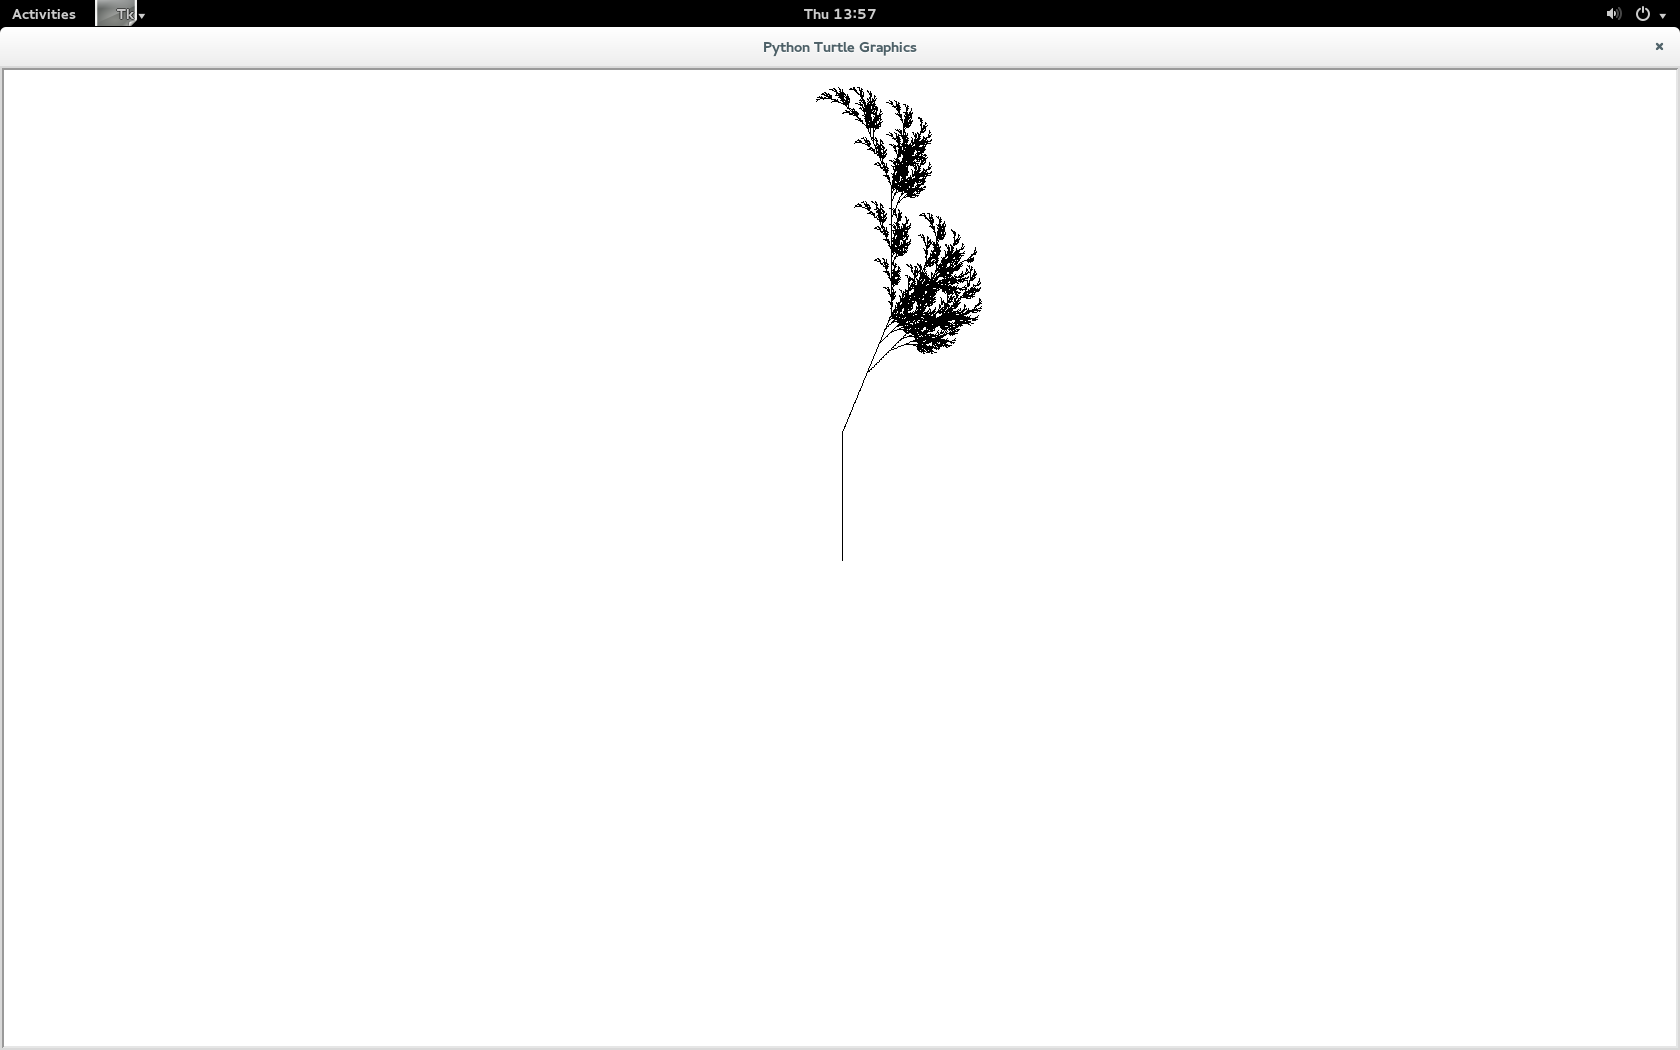
\includegraphics[width=0.75\textwidth]{fractal1.png}
\end{center}
\caption{Fractal 1\label{fig:gprun}}
\end{figure}

\begin{figure}[tbh]
\begin{center}
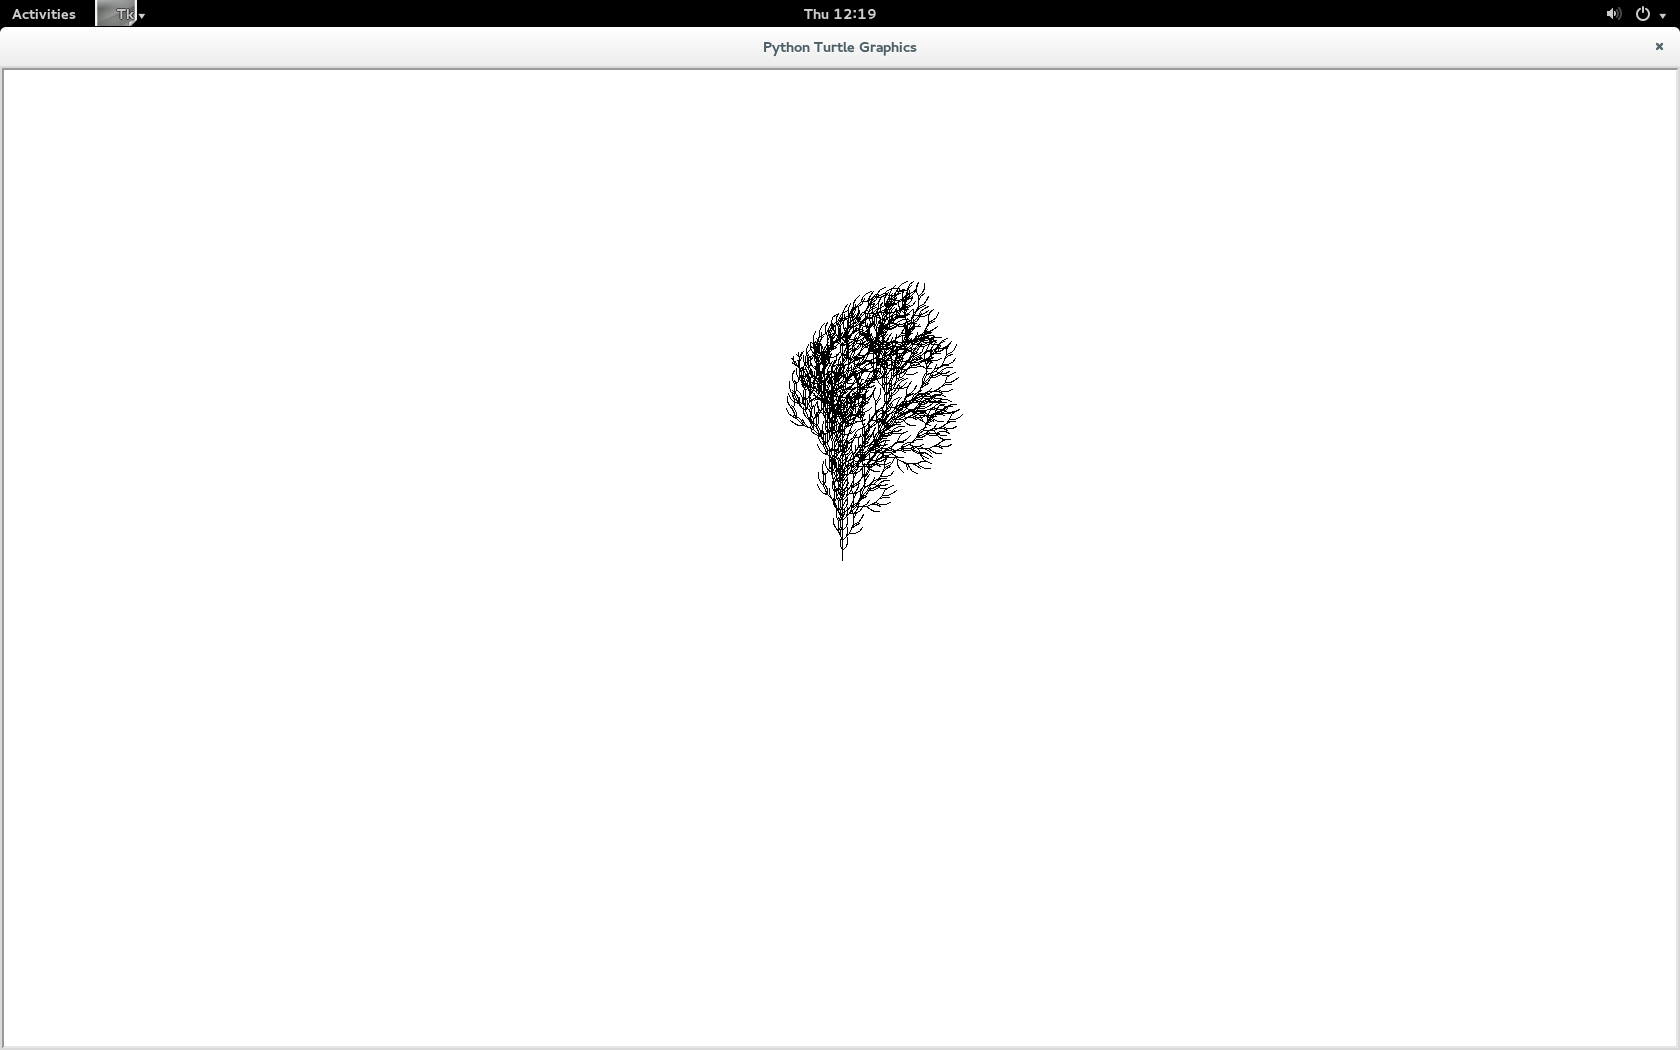
\includegraphics[width=0.75\textwidth]{fractal2.png}
\end{center}
\caption{Fractal 2\label{fig:gprun}}
\end{figure}

\begin{figure}[tbh]
\begin{center}
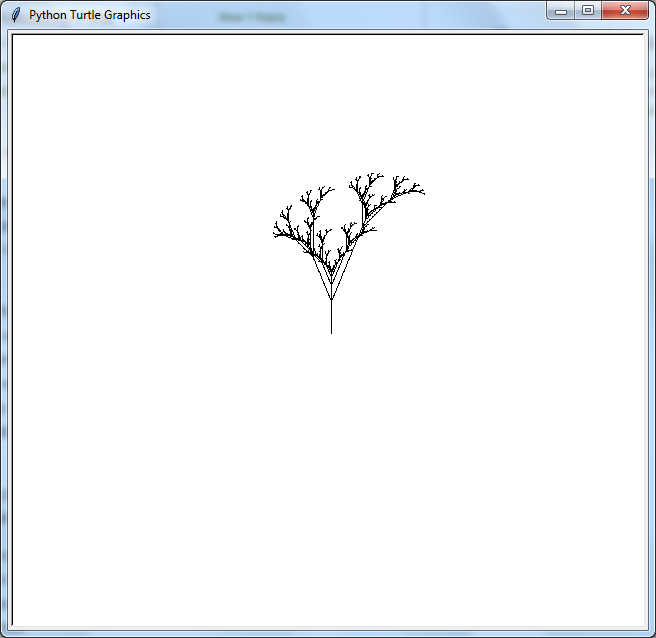
\includegraphics[width=0.75\textwidth]{fractal3.png}
\end{center}
\caption{Fractal 3\label{fig:gprun}}
\end{figure}

\begin{figure}[tbh]
\begin{center}
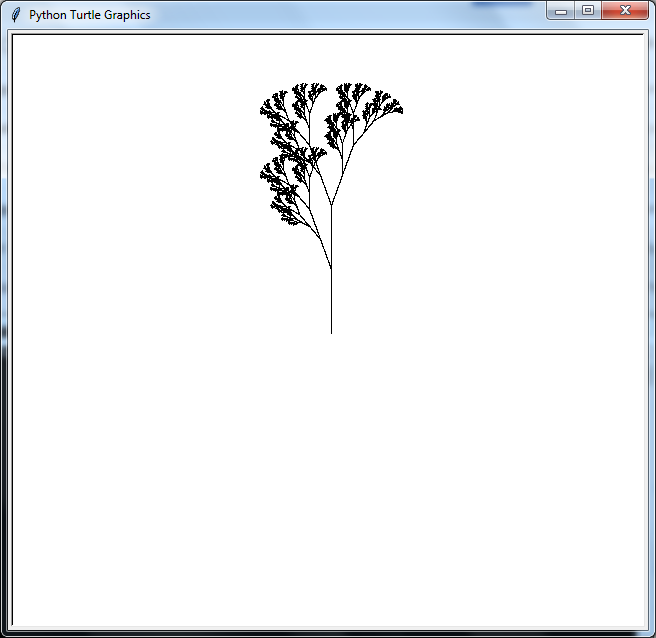
\includegraphics[width=0.75\textwidth]{fractal4.png}
\end{center}
\caption{Fractal 4\label{fig:gprun}}
\end{figure}	

\begin{figure}[tbh]
\begin{center}
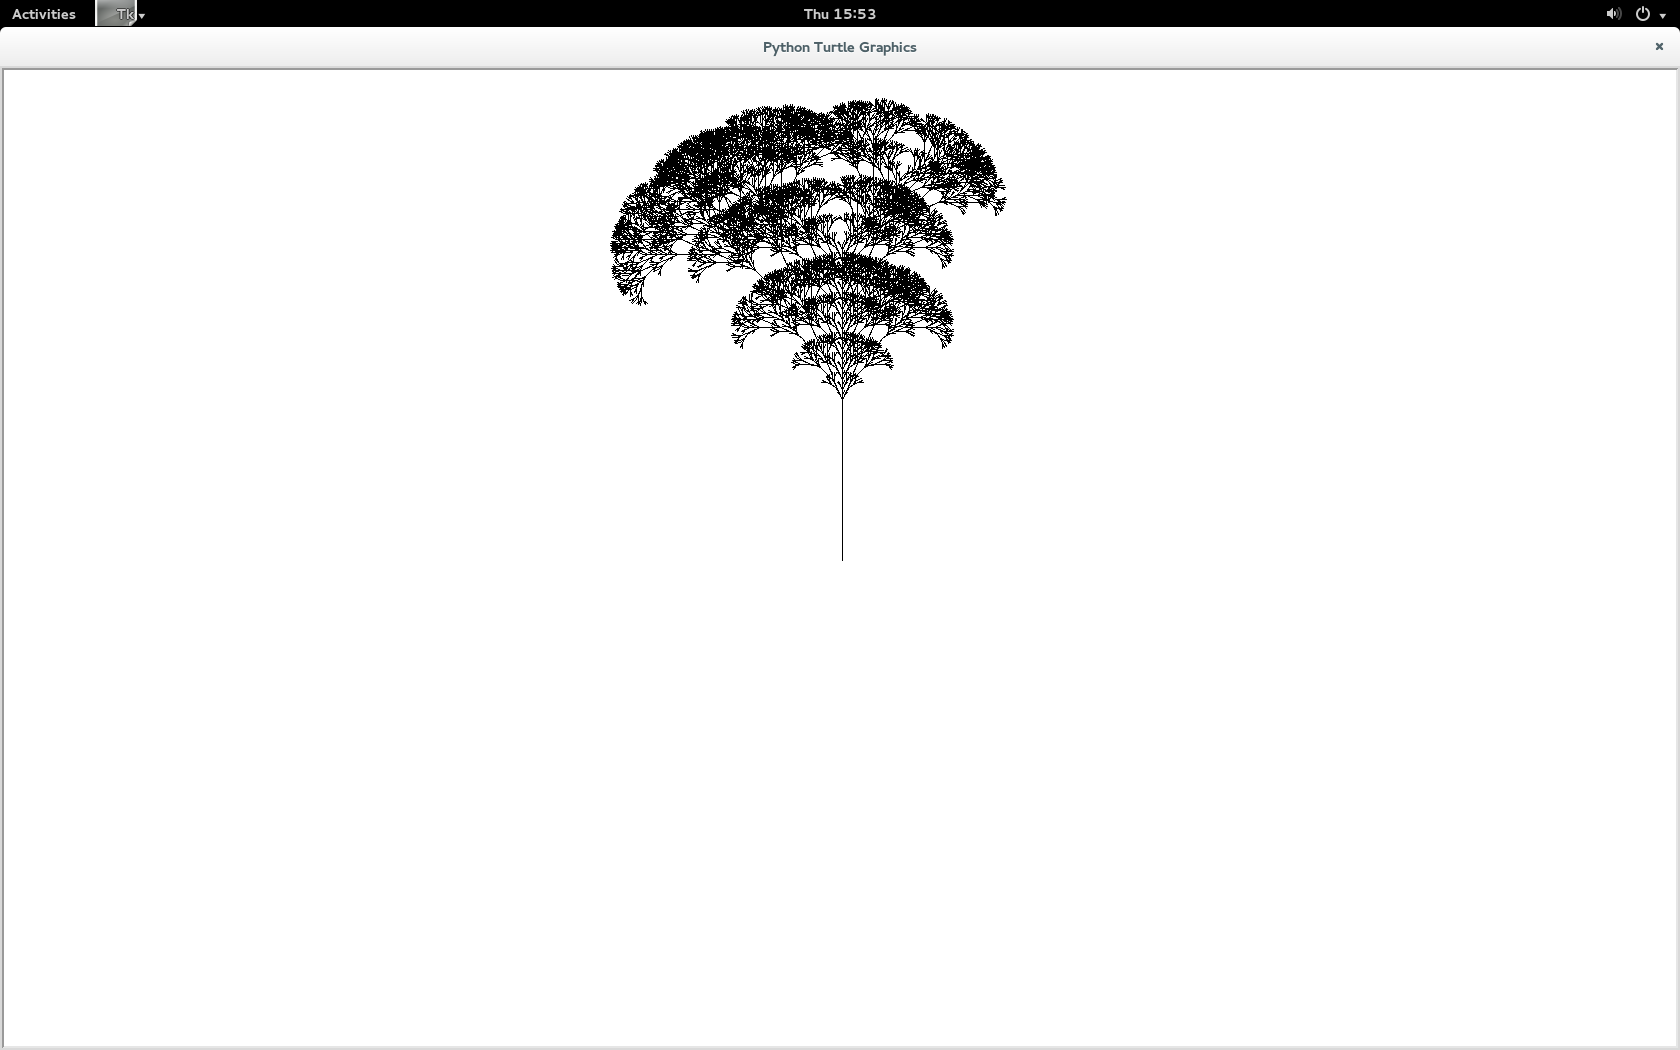
\includegraphics[width=0.75\textwidth]{fractal6.png}
\end{center}
\caption{Fractal 6\label{fig:gprun}}
\end{figure}
	


\section{Problem 7.15}

Implement a RIFS to generate all the fractals whose codes are presented in Table 7.3

\subsection{Problem Information}

RIFS - Random Iterated Function Systems - are a method of sequentially drawing fractals which give varying results.  Each iteration has a certain chance of making an affine transform on the current pixel and then updating the pixel to that transformed one.

Although RIFS systems are quite small code-wise, they can generate some very interesting shapes through emergent behaviour.  Table 7.3 presented us with some classic fractals: The Serpinski Gasket, the Bernoulli Fern, The Square and The Tree.  There was an error in the gasket's d column values - they should all be .5.

One major difference between the RIFS and IFS fractal generation systems is that while the IFS uses subimages or drawing strokes, the RIFS just uses individual pixel values.  This makes the turtle a poor fit for output, and so instead we used pyplot's scatter graph.  The results were simply lovely.

\subsection{Algorithm Description}

The RIFS algorithm we implemented came straight out of the book.  The only real addition - other than the display functionality - was some user-friendly file parsing.  The first three values in the input file are the start point coordinates of the fractal followed by the point size.  The larger the point size, the denser the fractal is drawn.

The fractal building took the initial point, and then selected an affine transform loaded from the table file via roulette wheel selection.  The p column in the file - the last column, that is - specified the chance that any given transform would be applied.

After an affine transform was randomly picked, so that the selected column j was chosen, a function was called which pulled the table values at that specified j into some transformation matrices, which were then multiplied with the current point.  The resultant point was returned and then drawn to the screen, and the loop restarted.  It ended when the maximum number of iterations was reached.

\subsection{Results}

Despite using such a simple, straightforward implementation, our results were exceedingly good.  A great number of iterations to use is actually 1000000.   A percentage is updated on the console as the fractal is built, and then the fractal will take a while to draw.  The result is a nicely drawn fractal in a proportionally square plot.


\begin{figure}[tbh]
\begin{center}
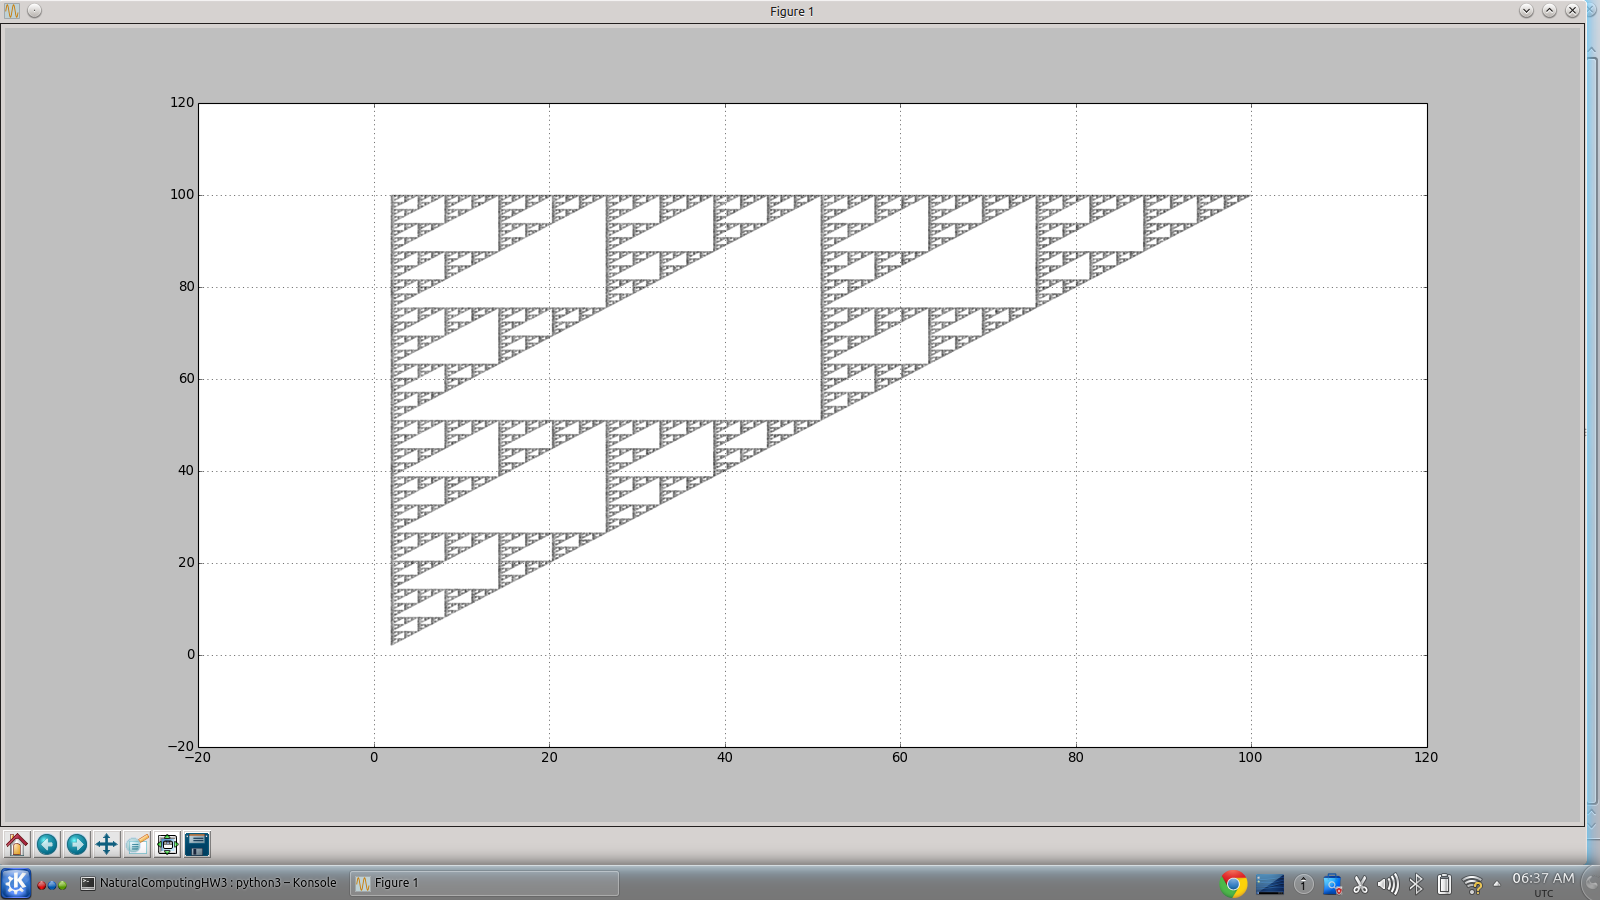
\includegraphics[width=0.75\textwidth]{s_gasket.png}
\end{center}
\caption{The Serpinski Gasket\label{fig:gprun}}
\end{figure}

\begin{figure}[tbh]
\begin{center}
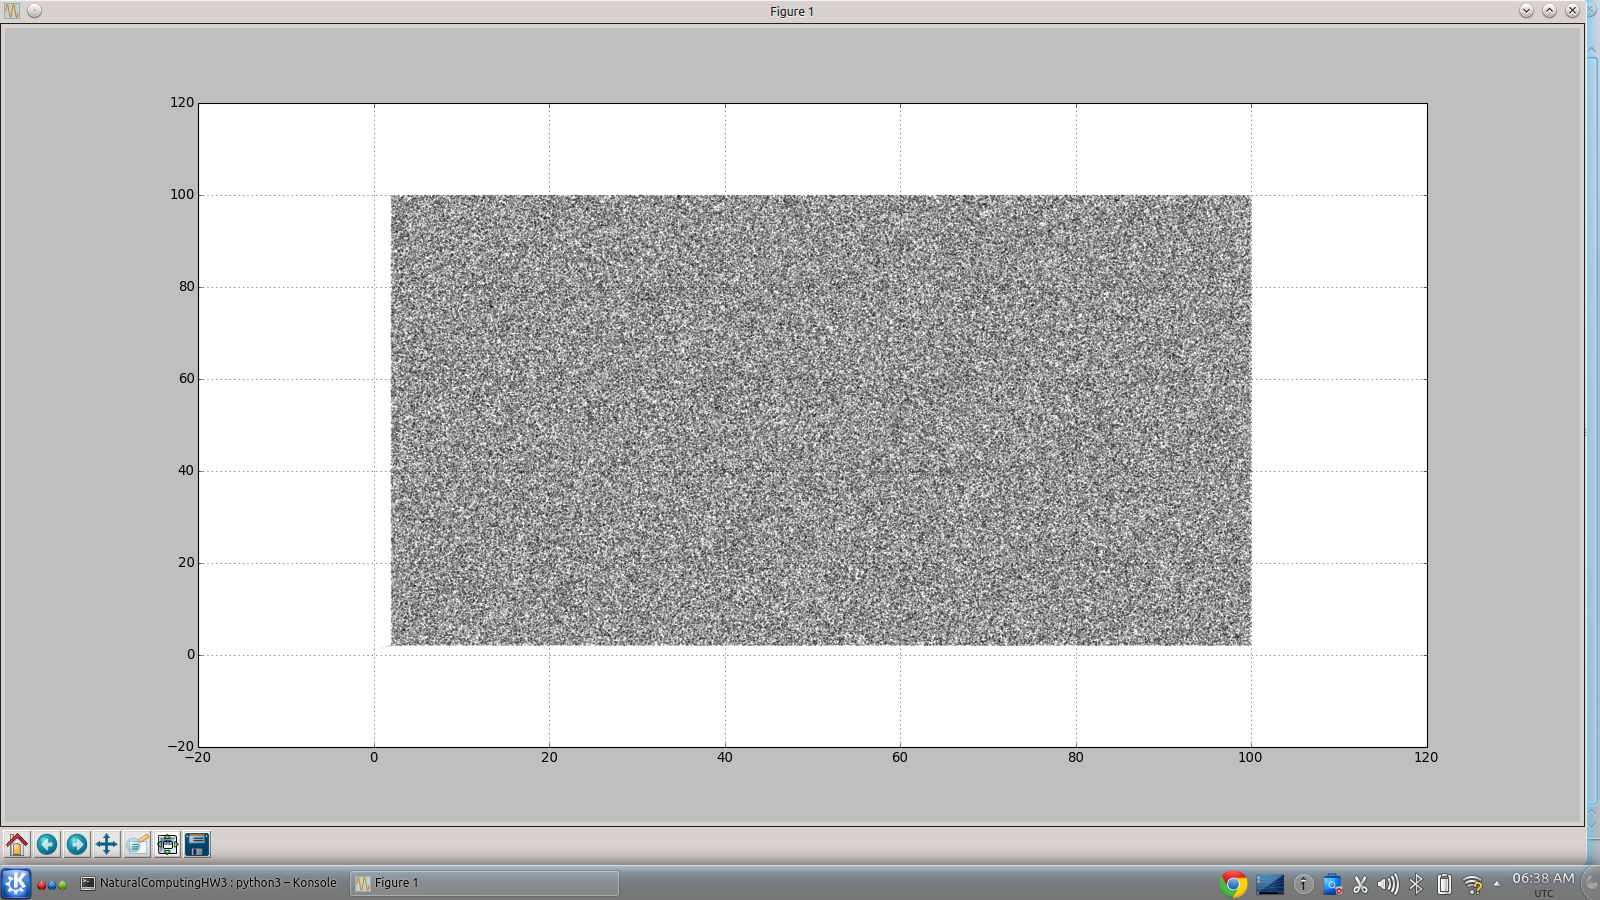
\includegraphics[width=0.75\textwidth]{square.png}
\end{center}
\caption{The RIFS square\label{fig:gprun}}
\end{figure}

\begin{figure}[tbh]
\begin{center}
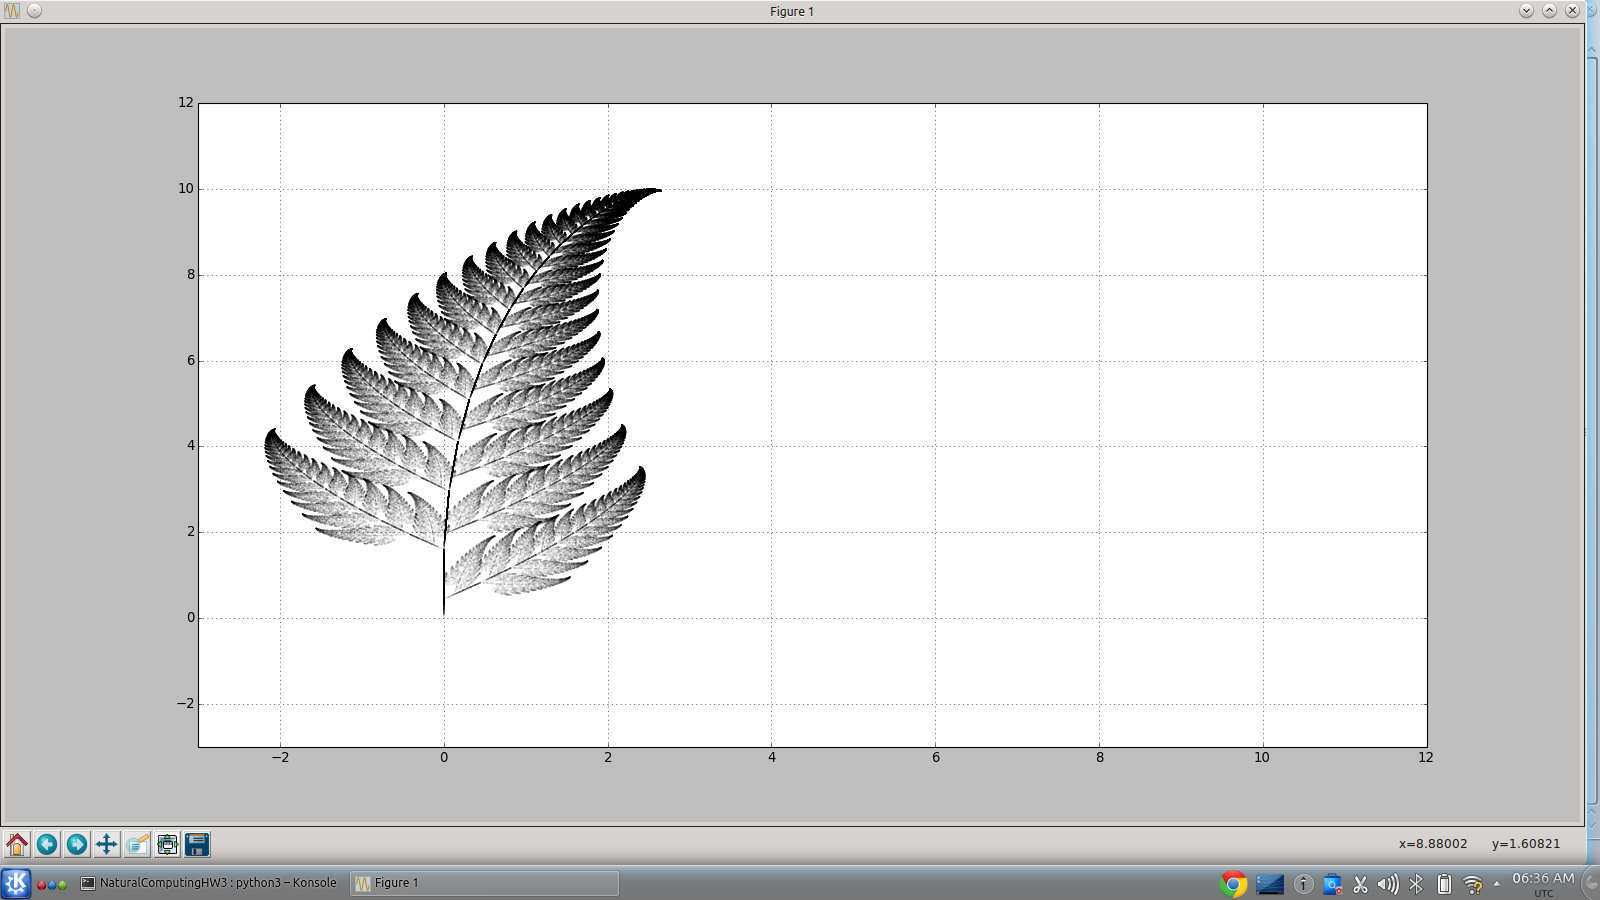
\includegraphics[width=0.75\textwidth]{b_fern.png}
\end{center}
\caption{The Barnsley Fern\label{fig:gprun}}
\end{figure}

\begin{figure}[tbh]
\begin{center}
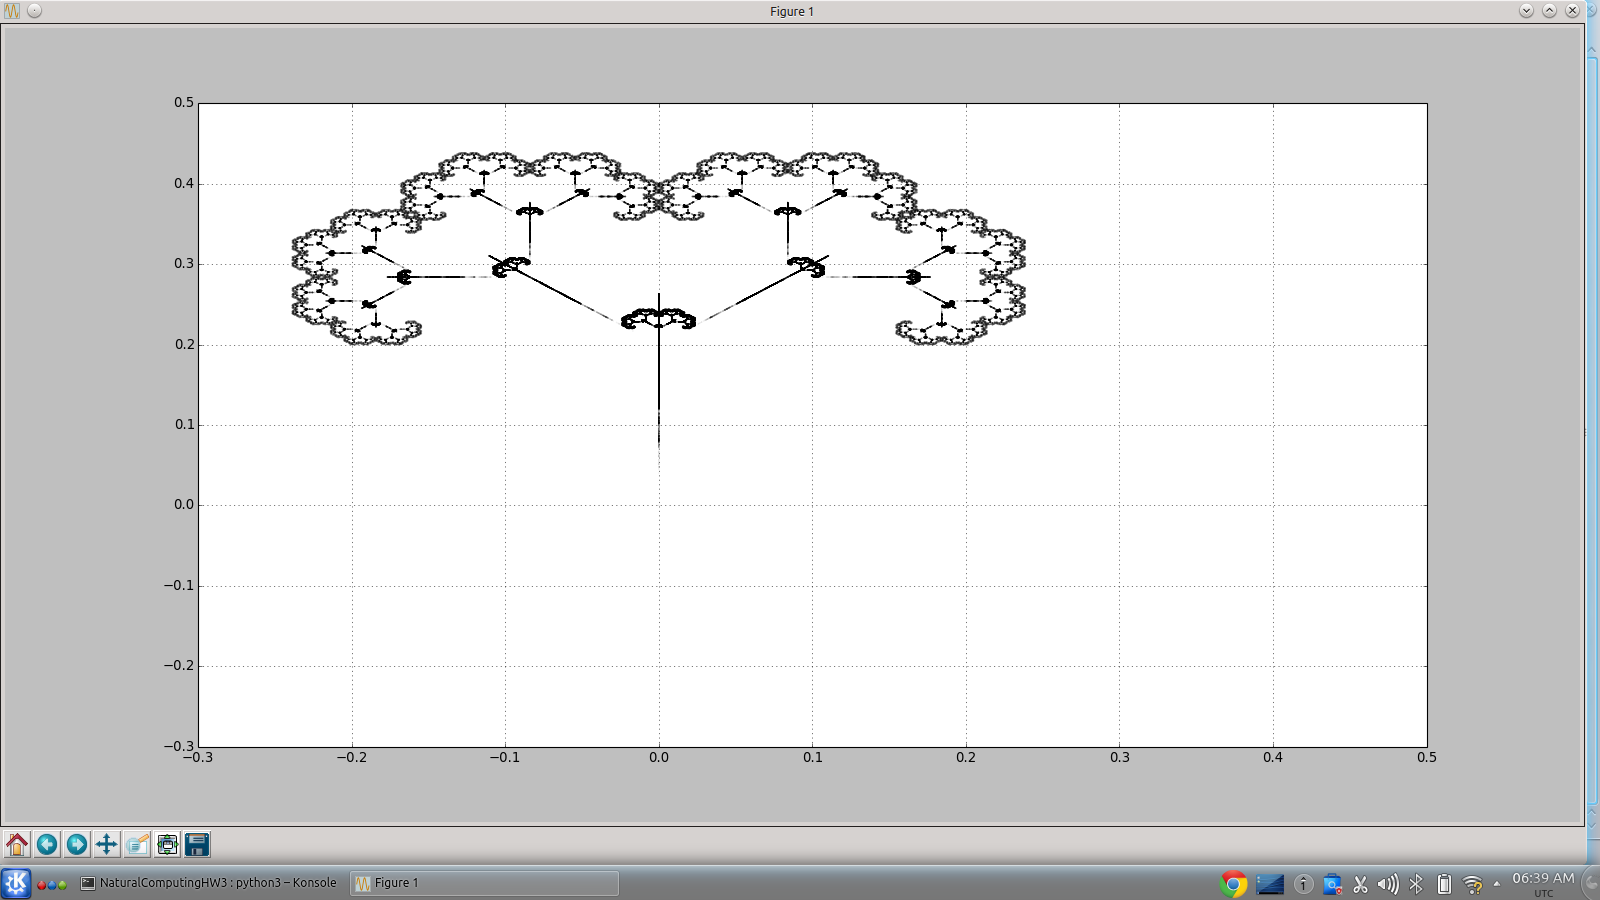
\includegraphics[width=0.75\textwidth]{tree.png}
\end{center}
\caption{The Tree\label{fig:gprun}}
\end{figure}



\section{Problem 7.21}

Implement the random midpoint displacement algorithm in 3D and generate some fractal landscapes.  Study the influence of the input parameters on the landscapes generated.

\subsection{Problem Information}

The midpoint displacement algorithm is a common method of generating fractal landscapes in 2D and 3D.  The book highlighted how to do it in 2D and gave some very explicit pseudocode for how to generate the landscapes with the algorithm.  It was up to us to extend it to 3D.

This problem required some drawn 3D output and a study of the input parameters, which were the number of divisions and the maximum deviation per iteration.  We shall refer to them as nmd and theta, respectfully.  The pyplot 3D axis object was used for generating the 3D landscapes, and the command line arguments specified the two input parameters.  Pyplot allowed the view to be rotated with the mouse.

\subsection{Algorithm Description}

Essentially, the algorithm has two parts: an iterative portion and a recursive portion.  The recursive portion builds a list of deltas - deviations - which depend on the division number and sigma.  They are stored for later and passed to the recursive function.  The recursive portion also requires a start and end point and number of divisions, along with the current division number.  It is called immediately after the delta list is built.

The recursive portion divides the distance between the two points in two and then sets its height to a random perturbation times the current division's detla value, which was calculated beforehand.  After the division, it returns if the current division is equal to nmd.  Else, it calls the next division on the midpoint between the two x values, the midpoint between the two y values, and the midpoint between the x and y values.  The result is a random landscape generally grading in one direction.

\subsection{Results and Analysis}

We are not terribly happy with the ugly results, although the algorithm appears to be working correctly.   Due to the poor fidelity of the 3D pyplot, it is very difficult to see much of anything unless large theta values are picked, and while the landscape is visible on the grid, the axis do not appear connected in the z-dimension, which is annoying.

An analysis on the input parameters is pretty basic.  When nmd is increased, the hills and vallies become smaller in radius and more numerous on the grid.  it also becomes exponentially slower, which makes sense.

When theta is increased, the hills and vallies become more pronounced.   If theta is too small, then the hills and vallies actually become invisible.  Due to the the nature of the algorithm, half of the hills and vallies are not visible at all unless the sigma is cranked up to a very high value.

As the code file says, a good trial run uses a width of 10, an nmd of 4 and a theta of 10.  

\begin{figure}[tbh]
\begin{center}
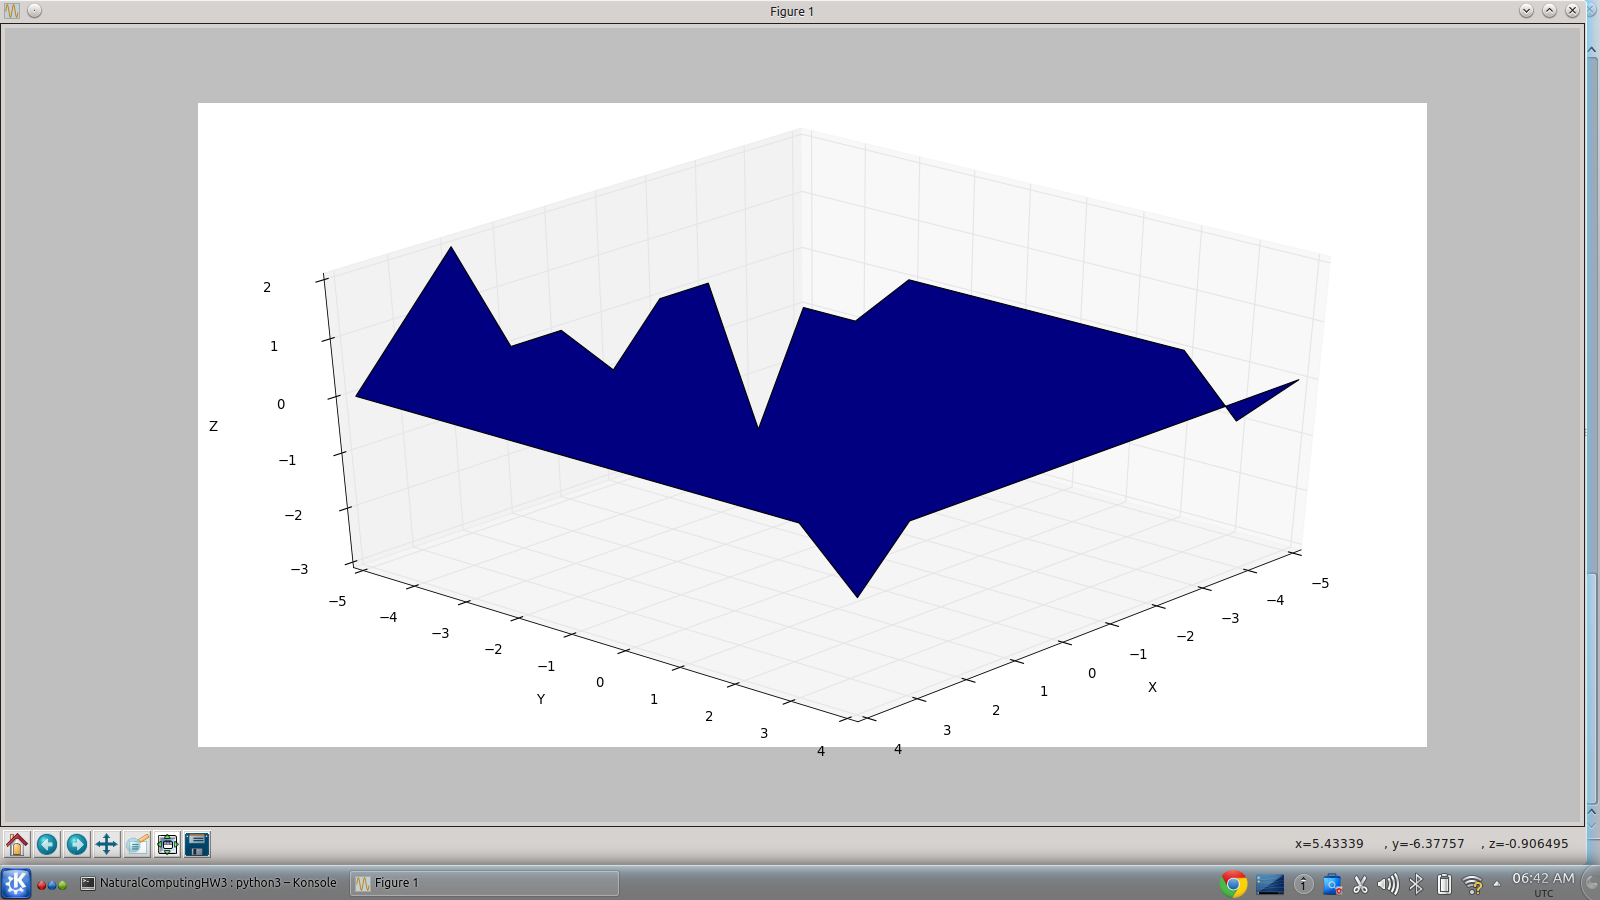
\includegraphics[width=0.75\textwidth]{landscape1.png}
\end{center}
\caption{A Simple Fractal Landscape\label{fig:gprun}}
\end{figure}

\begin{figure}[tbh]
\begin{center}
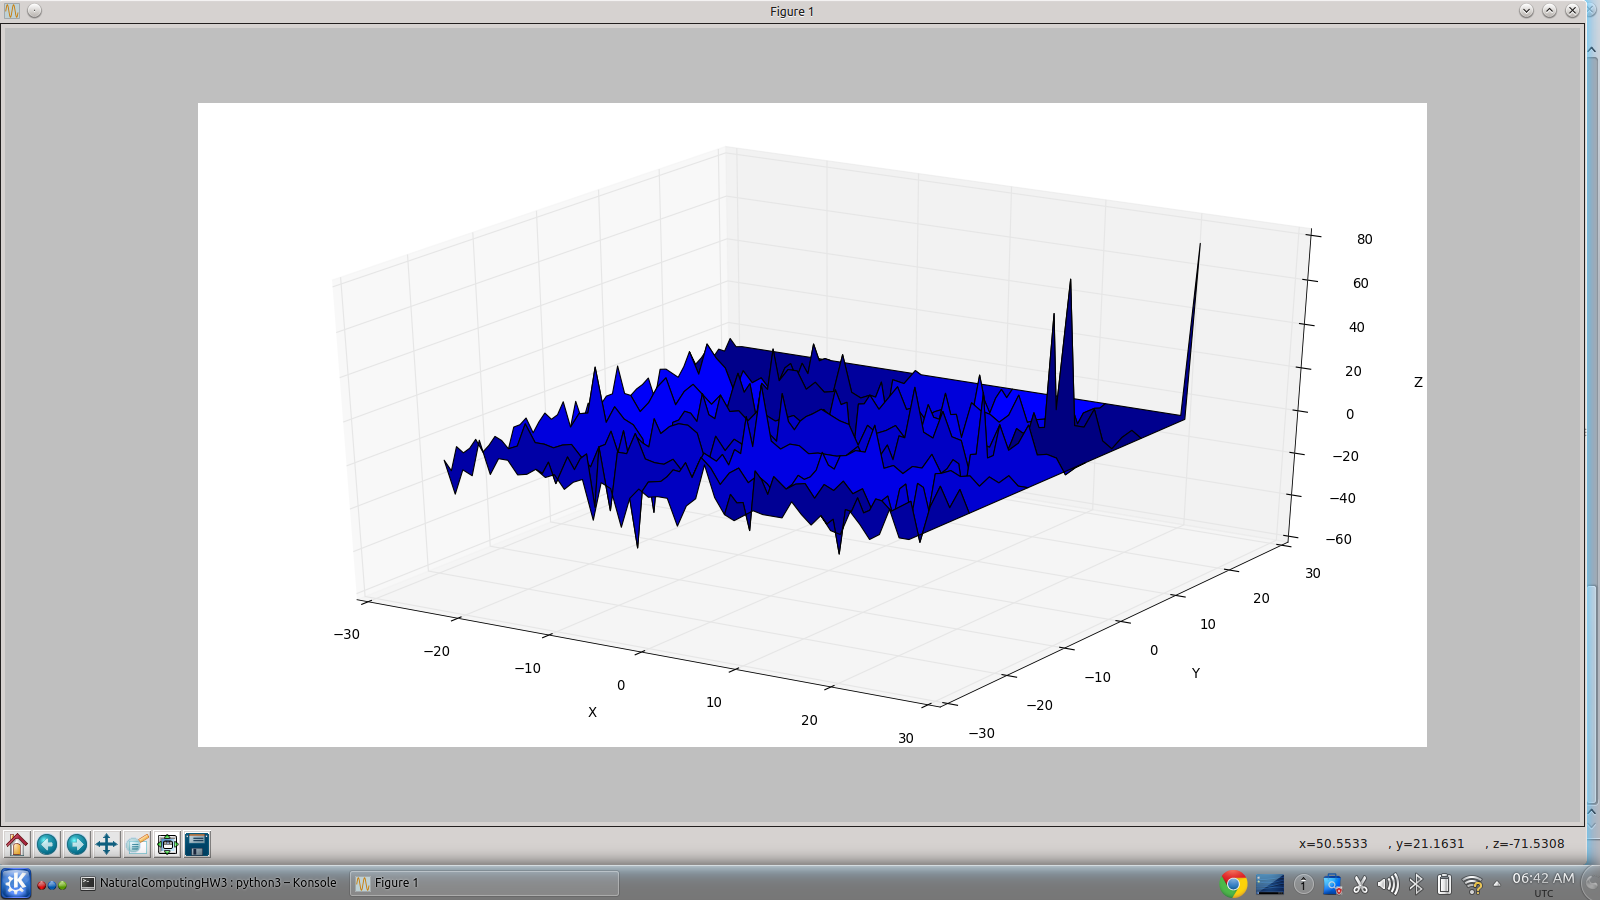
\includegraphics[width=0.75\textwidth]{landscape2.png}
\end{center}
\caption{A More Complex Fractal Landscape\label{fig:gprun}}
\end{figure}

% !TEX root = BioInspired.tex

\chapter{Slides - Heat Flow}

\section{Problem}

	Implement the heat flow diagram in the text using an insulated top and bottom layer.  

\subsection{Implementation}

	Using python and the matplotlib module, I used Dr. McGough's code from the slides to implement the diagram.  Working in the OPP lab however the computers there did not have the matplotlib installed, so I had to resort to using Python 2 rather than Python 3 which didn't appear to affect the final result much at all, if any.

\subsection{Issues}

	Like I said, the computers in the linux lab did not have matplotlib installed so Python 3 would not run the code.  Python 2 was used instead to fix this.

\subsection{Analysis}

	Aside from the Python 2, Python 3 issues, this program was very easy to implement mostly because all of the code was from the slides, except for the two if statements I added for the insulation.  Overall it turned out well and illustrated the heat flow accurately.

\begin{figure}[tbh]
\begin{center}
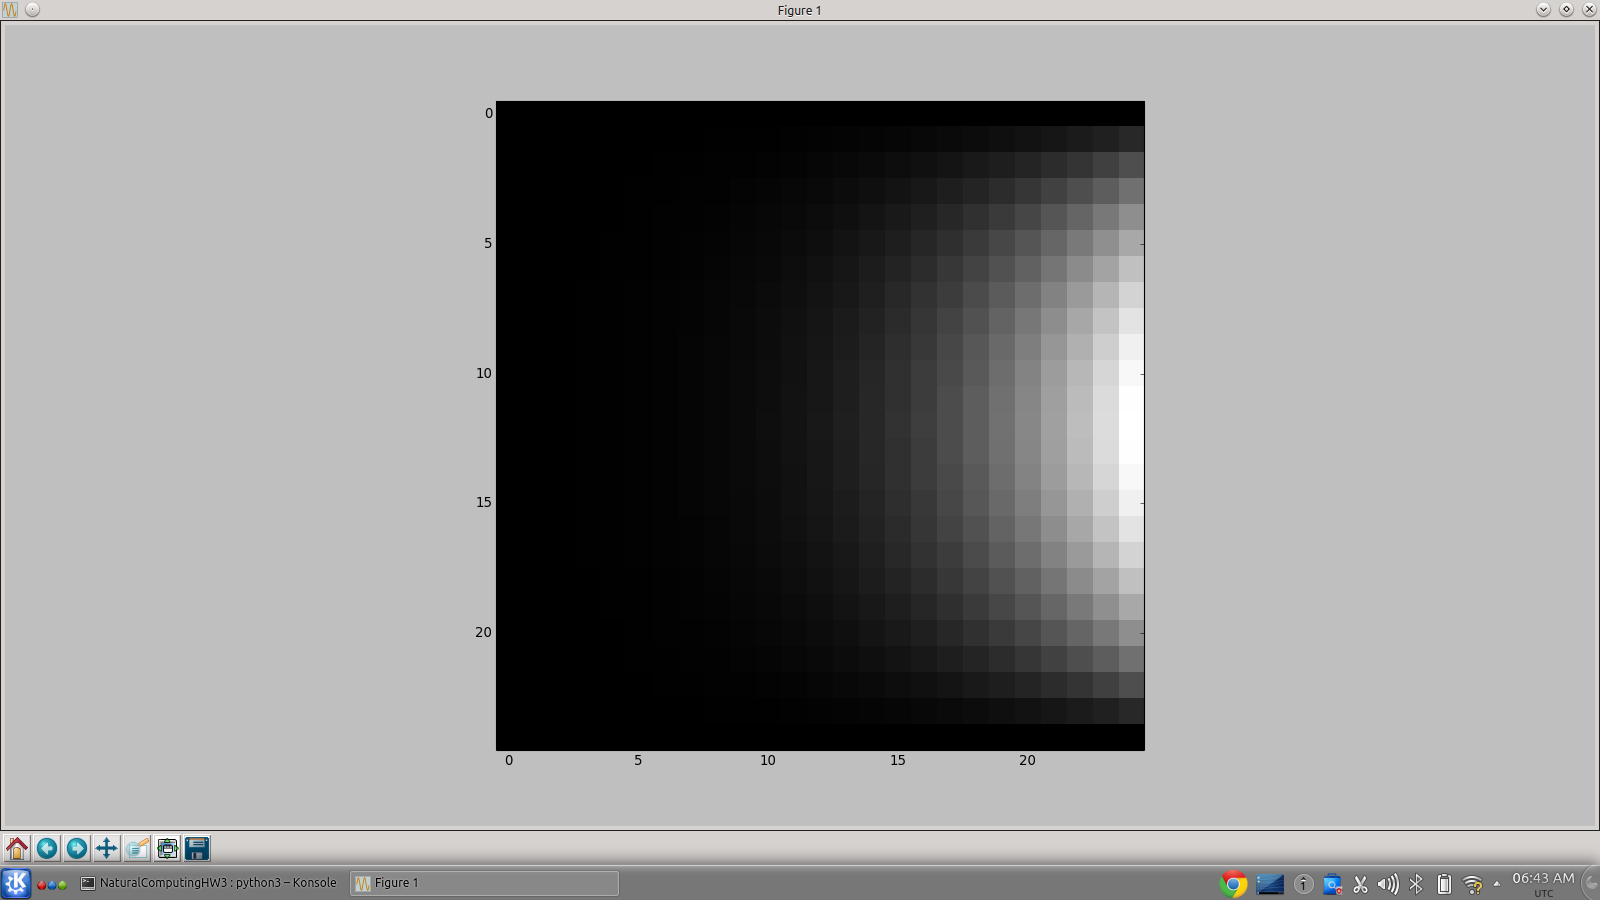
\includegraphics[width=0.75\textwidth]{heatflow.png}
\end{center}
\caption{The Heat Flow Visualization\label{fig:gprun}}
\end{figure}

% !TEX root = BioInspired.tex

\chapter{Immunocomputing - Text Chapter 6}

\section{Problem 6.1}

Use a bone marrow algorithm to define genes for gene libraries to be used to generate the inital population of a genetic algorithm to solve the TSP presented in CH 3 and CH 5 (figure 6.24).

\subsection{Problem Information}

As described, this problem requested that we generate an initial population for a genetic algorithm to use when solving the travelling salesman problem depicted in figure 6.24 in the book.  It also elaborated upon the description with the following (paraphrased):


Gene length Lg = 4, number of libraries n = 8, and library length (number of genes in each library) Ll = 4.  As one gene from each library will be selected, the total chromosome length is L = Lg x n = 4 x 8 = 32, that corresponds to the number of cities in a tour.


Each gene will be defined as a sequence of four cities known to be part of an optimal route.


A repair algorithm must be used in order to generate permutations of L integers while maintaining most of the genes intact.  This is because the TSP problem has the contraint that no city can be visited more than once.  to illustrate this problem and one possible way of solving it, consider the example presented in figure 6.25 in the book.

\subsection{Algorithm Description}

Bone marrow algorithms are simple techniques used primarily to build antibodies out of gene libraries for artificial immune systems.  Generally, they can also be utilized to build genomes out of a collection of random genotypes stored in such a gene library.


Building a list of cities using the bone marrow algorithm was straightforwards.  First of all, we began by creating a random set of gene libraries by randomly sampling stretches of cities (of length 4, of course) from a hardcoded optimal route, as specified in the problem.  Next, we used these gene libraries to build enough routes to fill a population, taking a random stretch of cities from each gene library per route.  After each route was built, however, we applied a repair algorithm in order to fit the constraints of the travelling salesman problem. This involved replacing all repeated cities with randomly ordered cities which were unused before the repairing.  In the end, the python script prints out all routes in the initial population.  If one were to then implement a GA for the travelling salesman problem, the population could be used to begin selection and breeding.

\subsection{Results}

As it was outside of the scope of the problem, we did not evaluate the routes generated by the bone marrow algorithm.  However, the variety was apparent while the stretches of pre-built genes were clearly present in the genomes. 
% !TEX root = BioInspired.tex

\chapter{Cellular Automata - Text Chapter 8}

\section{Problem 8.3}

Implement one of the Problems on the StarLogo website -- we chose to do the rabbit and grass simulation.

\subsection{Problem Information}

The rabbit and grass simulation proposes a plane with randomly scattered grass and rabbits.  Over time, the patches without grass grow grass and the rabbits move around, eating the grass off of the grassy patches.  As the rabbits consume the grass, they gain energy.  Once they reach a sufficient energy level, they bud off a second rabbit, which goes off on its own and eatis and reproduces by itself.

The Rabbits all move randomly and lose a slight amount of energy with every movement.  If they run out of energy, they die.

There are a handful of parameters which can be passed into the simulation.  The hatch threshold is the amount of energy required for reproduction in a single rabbit.  The starvation rate is the amount of energy that bunnies lose at every movement.  The grass growth rate is the chance that grass will grow in any given square in any given time step.  The maximum iterations is the maximum number of steps that the simulation will run.

\subsection{Algorithm Description}

We created a Bunny class, which held the position and energy of the bunnies.  In the time step, the grass matrix was updated by growing grass in each tile with a certain probability.  However, before the grass was grown, the bunnies were iterated through.  Their various bodily functions and movements were processed and their energy was modified, and then at the end of each bunny's iteration, it would be marked as dead if its energy

was below zero.  At the end of the time step, all bunnies which were marked as dead were removed.  At the end of each step, the pyplot was updated with the grass and grassless spots, drawing red spots where there were bunnies.

\subsection{Results}

This was simple and fun, and different settings yielded very different results.  Setting the starvation rate to something very low - like .05 - and setting the growth rate to something also very low - like .001 - give a good example of a fluctuating population.  The default parameters give a fairly generic example.  If the growth rate was too high in relation to the starvation rate, then the bunnies would exponentially overpopulate.  If the converse was
 true, then the rabbits would go extinct.  Decreasing the hatch threshold speeds up the whole simulation.
  




\section{Problem 8.4}

Implement Conway's Game of Life

\subsection{Problem Information}

Conway's Game of Life is a well-known cellular automata simulation of which Derek was already familiar.  This made testing and verification easy, although the main challenge was in implementing a fast solution.  

Conway's Game of Life is a simulation with four simple rules.  Firstly, any cell with more than three live neighbors dies of overcrowding.  Secondly, any cell with exactly three neighbors comes to life.  Thirdly, any cell with less than two neighbors dies of starvation.  Lastly, any live cell with two or three neighbors lives on to the next generation.

\subsection{Algorithm Description}

We implemented a grid which was drawn by pyplot, setting live cells to black and dead cells to white.  Following each of those rules iteratively, we updated the cell grid each generation.  

The number of neighbors for each cell was calculated by convolving the grid with a 3x3 mask.

\subsection{Results}

The result was an adjustable game of life accurate to the specifications.   The first argument should be start.txt, the second should be the generations/second - 10 is usually good.  The third argument should be the maximum number of generations, which is entirely up to the user.  Entering a very high number is advised. The starting configuration file is structured so the first line has the height and width of the playing field Subsequent lines are rows in the playing field.  0s are cells which are dead, and 1s are cells which are alive.
% !TEX root = BioInspired.tex

\chapter{Immunocomputing - Text Chapter 6}

\section{Problem 6.1}

Use a bone marrow algorithm to define genes for gene libraries to be used to generate the inital population of a genetic algorithm to solve the TSP presented in CH 3 and CH 5 (figure 6.24).

\subsection{Problem Information}

As described, this problem requested that we generate an initial population for a genetic algorithm to use when solving the travelling salesman problem depicted in figure 6.24 in the book.  It also elaborated upon the description with the following (paraphrased):


Gene length Lg = 4, number of libraries n = 8, and library length (number of genes in each library) Ll = 4.  As one gene from each library will be selected, the total chromosome length is L = Lg x n = 4 x 8 = 32, that corresponds to the number of cities in a tour.


Each gene will be defined as a sequence of four cities known to be part of an optimal route.


A repair algorithm must be used in order to generate permutations of L integers while maintaining most of the genes intact.  This is because the TSP problem has the contraint that no city can be visited more than once.  to illustrate this problem and one possible way of solving it, consider the example presented in figure 6.25 in the book.

\subsection{Algorithm Description}

Bone marrow algorithms are simple techniques used primarily to build antibodies out of gene libraries for artificial immune systems.  Generally, they can also be utilized to build genomes out of a collection of random genotypes stored in such a gene library.


Building a list of cities using the bone marrow algorithm was straightforwards.  First of all, we began by creating a random set of gene libraries by randomly sampling stretches of cities (of length 4, of course) from a hardcoded optimal route, as specified in the problem.  Next, we used these gene libraries to build enough routes to fill a population, taking a random stretch of cities from each gene library per route.  After each route was built, however, we applied a repair algorithm in order to fit the constraints of the travelling salesman problem. This involved replacing all repeated cities with randomly ordered cities which were unused before the repairing.  In the end, the python script prints out all routes in the initial population.  If one were to then implement a GA for the travelling salesman problem, the population could be used to begin selection and breeding.

\subsection{Results}

As it was outside of the scope of the problem, we did not evaluate the routes generated by the bone marrow algorithm.  However, the variety was apparent while the stretches of pre-built genes were clearly present in the genomes. 

%%%  Done with chapters
% Bib stuff

%\bibliographystyle{plain}
%\bibliography{refs.bib}
%\addcontentsline{toc}{chapter}{Bibliography}


% chapters in backmatter don't have numbers, but they appear in the
% table of contents, and are numbered BM-X where X is the page number
% relative to where the backmatter begins.
\backmatter

%%  The author of LaTeX provided all of us with a sample document.  Here it is ...
%\chapter{\LaTeX\ Example}
%% !TEX root = BioInspired.tex


\LaTeX\xspace sample file:  

\section{Introduction}
This is a sample input file.  Comparing it with the output it
generates can show you how to produce a simple document of
your own.

\section{Ordinary Text}  % Produces section heading.  Lower-level
                                    % sections are begun with similar 
                                    % \subsection and \subsubsection commands.

The ends  of words and sentences are marked 
  by   spaces. It  doesn't matter how many 
spaces    you type; one is as good as 100.  The
end of   a line counts as a space.

One   or more   blank lines denote the  end 
of  a paragraph.  

Since any number of consecutive spaces are treated like a single
one, the formatting of the input file makes no difference to
      \TeX,         % The \TeX command generates the TeX logo.
but it makes a difference to you.  
When you use
      \LaTeX,       % The \LaTeX command generates the LaTeX logo.
making your input file as easy to read as possible
will be a great help as you write your document and when you
change it.  This sample file shows how you can add comments to
your own input file.

Because printing is different from typewriting, there are a 
number of things that you have to do differently when preparing 
an input file than if you were just typing the document directly.  
Quotation marks like 
       ``this'' 
have to be handled specially, as do quotes within quotes: 
       ``\,`this'                  % \, separates the double and single quote.
        is what I just 
        wrote, not  `that'\,''.  

Dashes come in three sizes: an 
       intra-word 
dash, a medium dash for number ranges like 
       1--2, 
and a punctuation 
       dash---like 
this.

A sentence-ending space should be larger than the space between words
within a sentence.  You sometimes have to type special commands in
conjunction with punctuation characters to get this right, as in the
following sentence.
       Gnats, gnus, etc.\    % `\ ' makes an inter-word space.
       all begin with G\@.   % \@ marks end-of-sentence punctuation.
You should check the spaces after periods when reading your output to
make sure you haven't forgotten any special cases.
Generating an ellipsis 
       \ldots\    % `\ ' needed because TeX ignores spaces after 
                  % command names like \ldots made from \ + letters.
                  %
                  % Note how a `%' character causes TeX to ignore the 
                  % end of the input line, so these blank lines do not
                  % start a new paragraph.
with the right spacing around the periods 
requires a special  command.  

\TeX\ interprets some common characters as commands, so you must type
special commands to generate them.  These characters include the
following: 
       \$ \& \% \# \{ and \}.

In printing, text is emphasized by using an
       {\em italic\/}  % The \/ command produces the tiny extra space that
                       % should be added between a slanted and a following
                       % unslanted letter.
type style.  

\begin{em}
   A long segment of text can also be emphasized in this way.  Text within
   such a segment given additional emphasis 
          with\/ {\em Roman} 
   type.  Italic type loses its ability to emphasize and become simply
   distracting when used excessively.  
\end{em}

It is sometimes necessary to prevent \TeX\ from breaking a line where
it might otherwise do so.  This may be at a space, as between the
``Mr.'' and ``Jones'' in
       ``Mr.~Jones'',        % ~ produces an unbreakable interword space.
or within a word---especially when the word is a symbol like
       \mbox{\em itemnum\/} 
that makes little sense when hyphenated across 
       lines.

Footnotes\footnote{This is an example of a footnote.}
pose no problem.

\TeX\ is good at typesetting mathematical formulas like
       \( x-3y = 7 \) 
or
       \( a_{1} > x^{2n} / y^{2n} > x' \).
Remember that a letter like
       $x$        % $ ... $  and  \( ... \)  are equivalent
is a formula when it denotes a mathematical symbol, and should
be treated as one.

\section{Displayed Text}

Text is displayed by indenting it from the left margin.
Quotations are commonly displayed.  There are short quotations
\begin{quote}
   This is a short a quotation.  It consists of a 
   single paragraph of text.  There is no paragraph
   indentation.
\end{quote}
and longer ones.
\begin{quotation}
   This is a longer quotation.  It consists of two paragraphs
   of text.  The beginning of each paragraph is indicated
   by an extra indentation.

   This is the second paragraph of the quotation.  It is just
   as dull as the first paragraph.
\end{quotation}
Another frequently-displayed structure is a list.
The following is an example of an {\em itemized} list.
\begin{itemize}
   \item  This is the first item of an itemized list.  Each item 
          in the list is marked with a ``tick''.  The document
          style determines what kind of tick mark is used.

   \item  This is the second item of the list.  It contains another
          list nested inside it.  The inner list is an {\em enumerated}
          list.
          \begin{enumerate}
              \item This is the first item of an enumerated list that
                    is nested within the itemized list.

              \item This is the second item of the inner list.  \LaTeX\
                    allows you to nest lists deeper than you really should.
          \end{enumerate}
          This is the rest of the second item of the outer list.  It
          is no more interesting than any other part of the item.
   \item  This is the third item of the list.
\end{itemize}
You can even display poetry.
\begin{verse}
   There is an environment for verse \\    % The \\ command separates lines
   Whose features some poets will curse.   % within a stanza.

                           % One or more blank lines separate stanzas.

   For instead of making\\
   Them do {\em all\/} line breaking, \\
   It allows them to put too many words on a line when they'd 
   rather be forced to be terse.
\end{verse}

Mathematical formulas may also be displayed.  A displayed formula is
one-line long; multi-line formulas require special formatting
instructions.
   \[  x' + y^{2} = z_{i}^{2}\]
Don't start a paragraph with a displayed equation, nor make
one a paragraph by itself.

\section{Build process}

To build \LaTeX\ documents you need the latex program.  It is free and available on all operating systems.   Download and install.  Many of us use the TexLive distribution and are very happy with it.    You can use a editor and command line or use an IDE.  To build this document via command line:

\begin{verbatim}
alta>  pdflatex SystemTemplate
\end{verbatim}
If you change the bib entries, then you need to update the bib files:
\begin{verbatim}
alta>  pdflatex SystemTemplate
alta>  bibtex SystemTemplate
alta>  pdflatex SystemTemplate
alta>  pdflatex SystemTemplate
\end{verbatim}

The template files provided also contain a Makefile, which will
make things much easier.  

\section*{Acknowledgment}
Thanks to Leslie Lamport.  




\end{document}
